\section{Durchführung}
\label{sec:Durchführung}
Es werden die Beugungsfiguren von zwei Einzelspaten und einem Doppelspalt aufgenommen mittels der Apparatur
in Abbildung \ref{fig:aufbau}.
\FloatBarrier
\begin{figure}
 \centering
 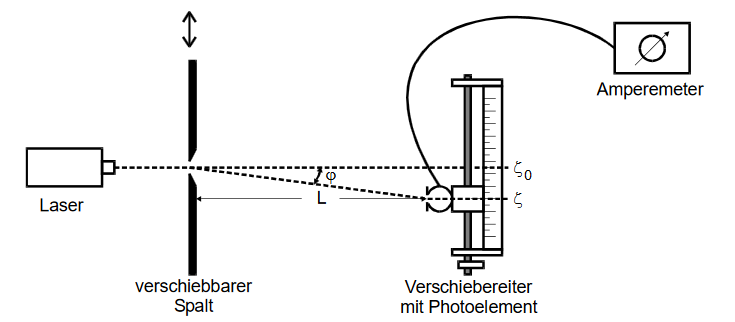
\includegraphics[width=0.6\textwidth]{aufbau.PNG}
 \caption{Apparatur zur Aufnahme der Beugungsbilder.\cite{sample}}
 \label{fig:aufbau}
\end{figure}
\FloatBarrier
Ein Helium-Neon-Laser stellt die Lichtquelle dar. Eine Photodiode registriert die Intensität und
gibt einen zur Intensität proportionalen Strom aus, welcher vom Amperemeter gemesssen wird.
Die Photodiode kann mittels Mikrometerschraube bewegt werden um die Abhängigkeit der Intensität vom Beugungswinkel
zu messen.
Ebenfalls werden alle Spaltbreiten mit dem Mikroskop gemessen.
